\chapter{Components}
\label{chap:components}
% we have described many technologies in previous cgapters
% for our architecture we have chosen the following technologies
% they will be discussed in greater details

% storage/persistent streeming/real time processing scala(or additional technologies/surrounding)

\authorsection{Storage systems}{SP}

\subsection{HDFS}

\subsection{Redys}

\authorsection{Real time processing systems}{SP}

\subsection{Storm}

\subsection{Scala}

\authorsection{Surrounding technologies}{SP}

\subsection{Spark}

\subsection{ZooKeeper}
When a distributed system becomes large and complicated, it needs a coorinator, that performs the system configuration management.
As it was mentioned in Chapter 4, Google uses a Chubby service for this purpose.
The main Chubby disadvantage is that for lock and unlock operations it is necessary to open and close the object consequently.
This feature influences the performance, increasing the time needed for making a lock.
Therefore Yahoo developes its own service named ZooKeeper that manages systems configuration and allows to efficiently lock the shared resources.

ZooKeeper provides a namespace that looks similar to a standard file system.
It consists of interconnected nodes, each of them identified by a path.
The path contains elements separated by a slash ('/').
Like in a file system, every node except the root has a parent node.
The parent node's path is a prefix for the current node path.
The ZooKeeper namespace differs from a standard file system in that its node can be a file and a directory simultaneously.

There are two types of nodes: persistent and ephemeral.
ZooKeeper stores persistent nodes on the disk, while ephemeral nodes belong to a particular session and exist only during this session.
Ephemeral nodes cannot have children nodes, they can only store data.
ZooKeeper client establishes a session with a ZooKeeper server, passing heartbeat messages.
When a client stopes to receive heartbeat messages, it reconnects to a defferent server, reestablishing the session.
If the session is canceled, all its ephemeral nodes are automatically removed.
ZooKeeper tree is presented in Figure~\ref{fig:zookeeper_tree} where the dark nodes are ephemeral.

\begin{figure}
  \centering
  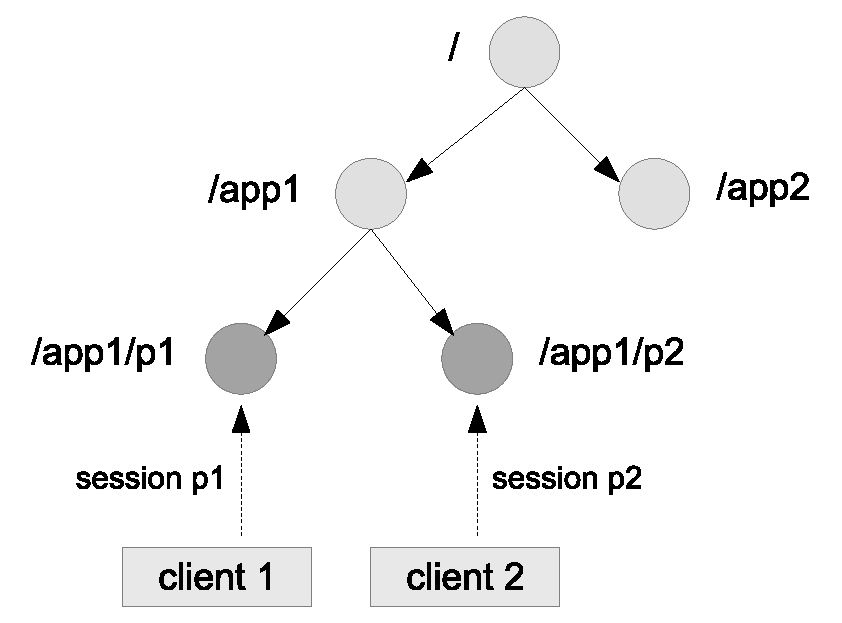
\includegraphics [width=0.9\textwidth]{images/zookeeper_tree}
  \caption{ZooKeeper tree sructure}
  \label{fig:zookeeper_tree}
\end{figure}

ZooKeeper is designed for small data warehousing, such as configuration, status and location information.
One node is usually not bigger than one kilobyte.
Therefore it stores data tree image in memory, keeping in a persistent store only transaction logs and snapshots.
In-memory storage limits the size of the database of ZooKeeper.
However, it gives advantages of low latency and high performance. 

The key feature of ZooKeeper is that it uses First In, First Out (FIFO) method for processing the messages.
It means that all commands are performed in the order they are received.
Thus, ZooKeeper maintains the total ordering.
The order is specified by a unique ZooKeeper Transaction id, that is assigned to each update.
 
ZooKeeper supports idempotent operations.
If a node should be updated, the system makes a note about the update and keeps an old and a new version of this node.
This allows client to receive the same message several times, being aware of when it can be applied.
Therefore all the write operations are performed sequentially in one thread on the master node.
However, the read request can be handled by a node's replica.
Moreover, the client also supports the total ordering of the messages.
Hence if the client sends a write request and then a read request, the write operation is performed first.
Even if usually read operation does not need a lock, ZooKeeper strictly follows the order.
It allows to implement predictable asynchronous systems that work with ZooKeeper.

The server part of ZooKeeper consists of one Leader and several Followers.
It uses two-phase commit protocol for processing updates.
During the first phase, the Leader attempts to prepare Followers to perform the steps needed to commit or abort a transaction.
This phase is also called voting phase, because the Leader receives the votes from the nodes, containing 'Yes' or 'No' reply.
In this case 'Yes' means commit and 'No' - abort.
During the second stage, the Leader performes a commit only if two of three Followers replyes 'Yes'.
Afterwards it notifies all the Followers about the result.

It can happened that one of the followers still has an outdated information when it receives the read request.
To avoid this problem, it is possible to make a force synchronisation with the master.
It is called the slow read.
Evidently, if all the clients use the slow read the system looses the advantage of scaling.
Without force synchronisation ZooKeeper system scales for reads nicely. 
However, in this case the client that reads from a replica can obtain the outdated information.

A client can watch a node.
If it sets a watch, it gets notified when the node is changed.
When the node sends this notification, it removes the watch.
In the case of connection problems between the client and the ZooKeeper server, the client receives a local notification.


\authorsection{Alternatives}{NO}